\section{\label{II-A-1}Une construction séparée : 25 ans d'évolution en silo}

L'histoire des \gls{thesaurus} au sein de l'établissement n'obéit pas à un plan concerté, mais résulte d'une sédimentation de pratiques, de logiciels et de métiers, ce qui a conduit à la formation de trois ensembles distincts de connaissances au musée : les \gls{thesaurus} de la bibliothèque gérés dans le logiciel \gls{alexandrie}, ceux des collections muséales gérés dans le logiciel \gls{micromusee}, et ceux de l'\gls{emediatheque}, gérés dans un logiciel de gestion dédié aux documents iconographiques et audiovisuels. Ces trois corpus de termes, bien que partageant une ambition commune – ordonner, nommer, rendre trouvable – ne sont pas nés du même mouvement ni selon les mêmes logiques. Chacun de ces trois ensembles est en réalité constitué de plusieurs \gls{thesaurus} ou listes d'\gls{autorite} distinctes, dont les plus importants sont ceux des mots-clés et des constructeurs d'aéronefs, qui se retrouvent dans les champs d'indexation des collections.

L'ensemble des informations recueillies au musée pour recréer un panorama des \gls{thesaurus} du musée et la méthodologie qui a été appliquée résultent pour la plupart de groupes de travail anciens ou de réflexions ponctuelles liées à des difficultés de description d'un objet en particulier. Celles-ci sont très rarement documentées, et lorsqu'elles le sont, elles sont difficiles à récupérer dans les archives du musée. Ce bref historique repose donc autant sur la mémoire des agents que sur les documents contemporains retrouvés\footnote{Voir l'interview de V. Dhorne en Annexe \ref{Ax-D}}.

\subsection{Les prémices : Alexandrie et Micromusée, une coexistence sans concertation (1996 – années 2010)}

Le premier \gls{thesaurus} à voir le jour semble avoir été celui de la bibliothèque, mis en place dès 1996. Conçu pour accompagner la structuration du catalogue et définir précisément les termes à utiliser pour les \glspl{autorite}, il répond aux exigences classiques du monde documentaire : classification rigoureuse, maîtrise du vocabulaire, liens hiérarchiques. Celui-ci s'inscrit dans une tradition de bibliothéconomie, qui est maîtrisée par les professionnels de la documentation. Parallèlement, en 2000, le logiciel \gls{micromusee} devient l'outil principal de gestion des collections muséales : il s'appuie sur une base propre, structurée différemment, dont la logique s'articule davantage autour des objets matériels que de concepts abstraits.

Des comités de pilotage\footnote{Voir l'interview de Vincent Dhorne en Annexe~\ref{Ax-D}} ont été organisés à partir 1998 entre les chargés de collections et les documentalistes autour du \gls{thesaurus}, notamment lors de l'import sur Micromusée des photos conservées par la bibliothèque. Cette instance a réuni des membres de la documentation, des chercheurs, ainsi que des chargés de collections invités à contribuer sur une base volontaire. Son objectif : poser les bases d'une politique de vocabulaire raisonnée, en définissant les différents \gls{thesaurus} existants, les références à utiliser, et la nomenclature à adopter. Selon les documents retrouvés dans les archives numériques du musée, ce comité se réunissait le premier lundi de chaque mois pour contrôler l'évolution du \gls{thesaurus} de \gls{micromusee}. Si l'on a du mal à dire aujourd'hui combien de temps il a duré, son existence témoigne d'une volonté initiale de coordination des vocabulaires à l'échelle du musée. Cependant, cette collaboration des métiers du musée autour de la formation d'un \gls{thesaurus} ne s'est pas concrétisée par des actions pour unifier les \gls{thesaurus} existants : malgré ce dialogue, ceux de la bibliothèque et du musée continuent à avoir une existence parallèle.

Ce double système, bien que fonctionnel dans chaque silo, met en lumière les défis liés à l'absence d'un langage documentaire commun, essentiel pour assurer la cohérence et l'efficacité des pratiques au sein de l'établissement. La question de la cohérence intellectuelle du musée, de la bibliothèque aux collections muséales, commence à se poser, la première réponse qui y est apportée est le dialogue, grâce à ces comités de pilotage. Cette solution intéressante ne semble pas avoir été appliquée assez longtemps ou assidûment pour répondre aux besoins actuels du musée, et son souvenir reste lointain voire inexistant dans la mémoire des agents.

\subsection{Un tournant documentaire : la création de l'\gls{emediatheque} (2016 – 2020)}

Un basculement s'opère autour de 2016 : le chargement des photographies dans \gls{micromusee} est délaissé au profit d'un nouveau dispositif, développé par et pour les documentalistes, l'\gls{emediatheque}. Cette plateforme dédiée aux documents iconographiques et audiovisuels permet un travail plus fin sur l'indexation, et elle est entièrement conçue pour ces collections de nature particulière. Depuis 2020, date de mise en ligne de l'\gls{emediatheque}, celle-ci est la référence pour l'indexation des images.

Avec ce nouveau logiciel, vient un nouveau \gls{thesaurus} : pour décrire ces collections spécifiques, il est choisi non pas d'en utiliser un déjà existant qui serait donc employé sur deux logiciels et pour deux catégories de collections différentes, mais d'en dériver de \gls{micromusee}. Celui-ci est enrichi de nouvelles entrées liées aux collections propres de l'\gls{emediatheque}, on lui ajoute de nouvelles listes d'\glspl{autorite}. Le dialogue avec la base \gls{micromusee} et les chargés de collections qui a été établi lors de la migration, ne perdure pas, et les deux \gls{thesaurus} entament dès lors deux évolutions séparées. Depuis au moins la période du Covid, aucun enrichissement réciproque n'a été mis en place, chaque \gls{thesaurus} du musée évoluant indépendamment, sans effort concerté pour un enrichissement commun. Aujourd'hui, les \gls{thesaurus} de \gls{micromusee} et de l'\gls{emediatheque} partagent donc une structure extrêmement proche, mais le second est devenu avec le temps bien plus fouillé et riche en termes que le premier -- auquel il a été fait moins d'ajouts que pour l'\gls{emediatheque}.

Ainsi s'installe une coexistence entre trois vocabulaires parallèles qui s'ignorent plus ou moins. Les \gls{thesaurus} de la documentation (\gls{emediatheque} et bibliothèque) sont utilisés par les mêmes personnes; enrichis suite à des processus de recherche similaires, les termes utilisés se ressemblent. Cependant, les règles d'indexations et de pratiques restent propres à chaque vocabulaire d'indexation plutôt qu'à tout le département. Le travail des documentalistes est reconnu, et leurs \gls{thesaurus} peuvent être consultés en cas de doute lors des évolutions sur les \gls{thesaurus} de description des collections muséales, mais nous n'avons pas recueilli de témoignage de l'action inverse. Progressivement, bien que les agents aient conscience de l'existence de ces \gls{thesaurus} et qu'ils les consultent ponctuellement pour retrouver un terme particulier, aucune réflexion générale n'a été menée avant cette année pour les penser comme un tout et rationaliser leur progression, qui est devenue dépendante des pratiques individuelles et de l'indexation de nouveaux objets.

\begin{figure}
	\centering
	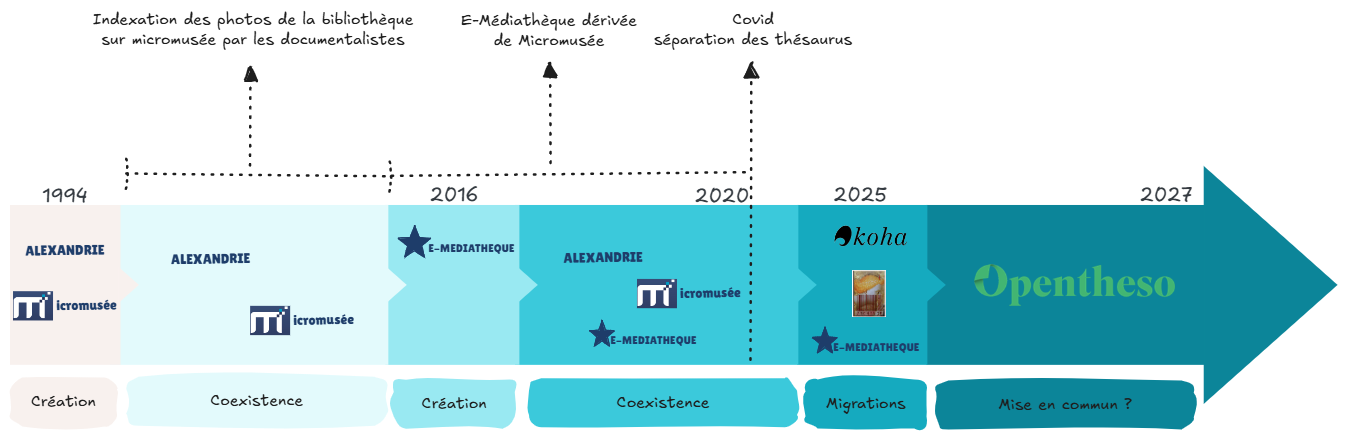
\includegraphics[width=0.9\linewidth]{img/FRISE_Thesaurus}
	\caption{Chronologie des logiciels et des ensembles de thésaurus utilisés au \mae depuis les années 1990.}
	\label{frise:thesaurus}
\end{figure}


\subsection{Des architectures hétérogènes}

Sur le plan technique, les divergences entre logiciels rendent toute interopérabilité complexe. Chaque base repose sur une architecture distincte; Alexandrie, en usage à la bibliothèque depuis 1996, a cédé la place en juillet 2025 à Koha, un logiciel libre structuré en MySQL, couplé à Clade pour la gestion documentaire. Le musée, de son côté, utilisait Micromusée (v6) depuis 2000, version qui a peu évolué depuis et dont les difficultés d'utilisation et l'ergonomie limitée ont certainement freiné la réflexion sur le \gls{thesaurus} qui était intégré. Ce logiciel a également été remplacé en juillet 2025 par Archange, une déclinaison du logiciel S-Museum développée pour les établissements du ministère des Armées. L'\gls{emediatheque}, développée pour les besoins du musée, reste quant à elle inchangée.

\begin{figure}[htbp]
	\centering
	\begin{subfigure}{0.45\textwidth}
		\centering
		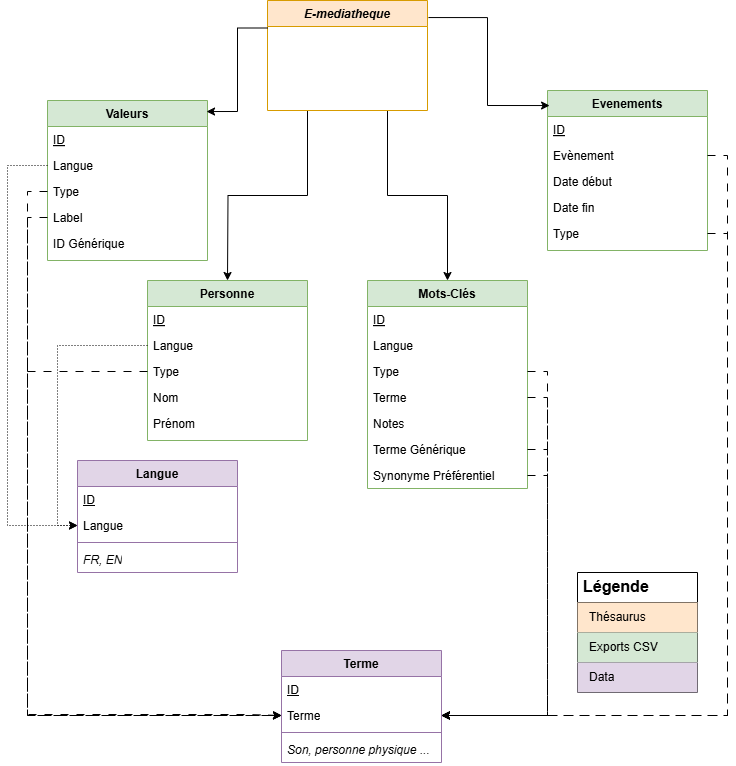
\includegraphics[width=\linewidth]{img/UML_emediatheque}
		\caption{Les \gls{thesaurus} de l'\gls{emediatheque}}
		\label{uml:emediatheque}
	\end{subfigure}
	\begin{subfigure}{0.45\textwidth}
		\centering
		\includegraphics[width=\linewidth]{img/UML_alexandrie}
		\caption{Les \gls{thesaurus} d'\gls{alexandrie}}
		\label{uml:alexandrie}
	\end{subfigure}
	\hfill
	\begin{subfigure}{0.5\textwidth}
		\centering
		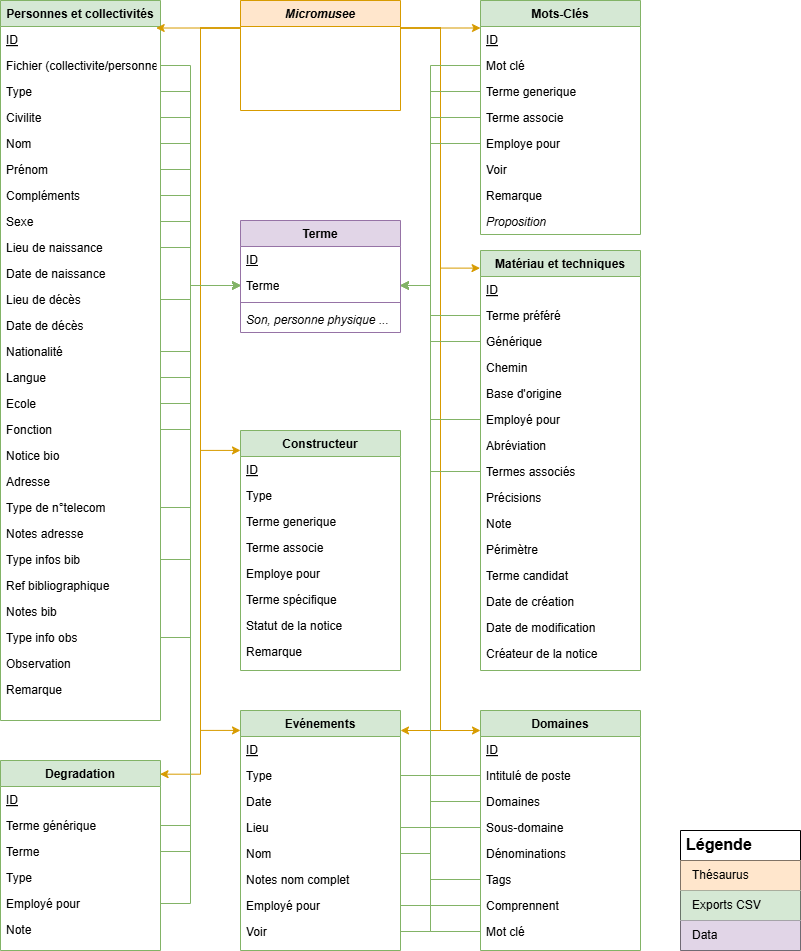
\includegraphics[width=\linewidth]{img/UML_micromusee}
		\caption{Les \gls{thesaurus} de \gls{micromusee}}
		\label{uml:micromusee}
	\end{subfigure}
	\caption[Construction des \gls{thesaurus} du \mae]{Trois ensembles de \gls{thesaurus} coexistent au \mae : ceux-ci présentent des familles de termes et des termes similaires, qui sont structurés différemment. Chacun d'entre eux est attaché à la description d'une certaine catégorie de collections, et présente ses richesses propres. On remarquera les similitudes entre l'\gls{emediatheque} et \gls{micromusee}, dont elle est dérivée.}
	\label{fig:thesaurusmusee}
\end{figure}


\bigskip

Ces outils ont été progressivement mis en place pour répondre aux besoins spécifiques des métiers et aux directives ministérielles : ils illustrent les défis de coordination et de standardisation dans le développement des \gls{thesaurus}. Ceux-ci respectent l'organisation générale recommandée en choisissant des termes descripteurs, leur attribuant des synonymes, les reliant à un ou plusieurs termes génériques et leur attribuant une définition, mais sans plus approfondir les possibilités décrites notamment dans les dernières normes ISO relatives à la gestion de \gls{thesaurus}. Celles-ci proposent en effet des méthodes pour unifier des \gls{thesaurus} existants, garantir leur interopérabilité indépendamment des systèmes et langages qui les hébergent et établir des ponts pour leur permettre de communiquer\footnote{\cite{chichereauNormesConceptionGestion2007}}, qui pourraient répondre aux exigences du musée.